\documentclass[10pt]{article}

\usepackage{multicol}
\usepackage[margin=0.75in]{geometry}
\usepackage{titlesec}
\usepackage{amsmath}
\usepackage[
backend=biber,
style=ieee,
sorting=ynt
]{biblatex}
\usepackage{fancyhdr}
\usepackage{enumitem}
\usepackage{graphicx}
\usepackage{float}

% \pagestyle{fancy}
%\fancyhf{}

\title{ECE419 M1 Report}
\date{28 January 2018}
\author{Thomas Kingsford\\Marcel Mongeon\\Zhihao Sheng}

%\titleformat{\section}{\normalfont\scshape}{\thesection}{1em}{}
%\titlespacing*{\section}{0pt}{10pt}{0pt}

%\setlength{\parindent}{0pt}
%\setlength{\parskip}{0cm}
%\renewcommand{\baselinestretch}{0.5}
%\setlist{noitemsep} % {nosep, noitemsep}

\begin{document}
\begin{multicols}{2}
\maketitle

\section{Design and Decisions}

\paragraph{Architecture} Refer to Figure \ref{arch} in the Appendices for an architecture diagram.

\paragraph{KVClient} The KVClient class handles client side interface. It creats a user interface which contains following operations:

\begin{enumerate}
    \item connect hostname port: establishing a connection to the host server with the port number.
    \item put key value: sending the key-value pair to the server which will store the pair.
    \item get key: getting the key-value pair with the key from the server.
    \item logLevel: setting the log level. The default level is OFF.
    \item disconnect: disconnecting from the current server.
    \item quit: quiting the application after disconnecting from the server.
\end{enumerate}

\paragraph{KVStore} The KVStore class handles the messages from the KVClient and passes them to the CommMod.

\paragraph{KVServer} The KVServer class handles server side interface. It gets the KVMessage from KVClient through the CommMod and does the put or get request, then it will give the response to the KVClient through the CommMode.

\paragraph{CommMod} The CommMod class handles client and server communications. The server registers as a listener and receives KVMessages by way of a callback. The server must respond to each received KVMessage with a response message. Clients Connect() then send messages via SendMessage(), which returns a KVMessage response or else times out if the server fails to respond quickly enough.

\paragraph{TLVMessage} The TLVMessage is an implementation of the KVMessage interface. it implements a modification of tag-length-value encoding. It (un)marshals a KV message as a sequence of bytes in which:

\begin{enumerate}
\item The first byte is the ordinal value of the StatusType enum, referred to as a 'tag'.
\item The second byte is the length of the key $L_K \in [0, 255]$. This protocol imposes an upper limit on key size of 255 bytes.
\item For messages containing a value (the existence of a value is fully determined by the tag), the third byte is the length of the value $L_V \in [0, 255]$. This protocol imposes an upper limit on key size of 255 bytes. This could be trivially extended - for instance, the use of four bytes would give a maximum length of $2^32-1\approx 1 \text{ billion bytes}$
\item The following $L_K$ bytes are the key.
\item If there is a value, the following $L_V$ bytes are the value.
\end{enumerate}

\paragraph{LRUCache} The LRUCache uses a LinkedHashMap implementation which, for every put operation, checks the total cache size and if greater than capacity will evict the entry which was accessed the longest time ago.

\paragraph{LFUCache} The LFUCache uses 2 HashMaps in order to store 1) the value to the key and 2) the usage counter. When a put is performed and the cache is becomes large then the enttry with the highest usage counter is removed from the cache.

\paragraph{FIFOCache} Similar to the LRUCache, the FIFOCache uses a LinkedHashMap implementation which, for every put operation, checks the total cache size and if greater than capacity will evict the entry which was inserted the longest time ago.

\paragraph{LockManager} The lock manager was designed so that locks can be acquired for a particular key, and to provide a timeout specified by the caller in the case a lock is not acquired. For all operations involving put from the KVServer/Cache, getKey(key, timeout) is called from the Cache. The key is then released by calling releaseKey(key), throwing an exception if the calling thread is not the owner. Per key locking is used in order to increase parallelized performance by ensuring that writes/deletes/updates are not blocked when threads are working on different keys.

\paragraph{FilePerKeyKVDB} The persistent storage implementation uses a simple storage mechanism by storing all key-value pairs in the same directory, but in seperate files. The file names are the k-v pair’s key and the file data is the value for that pair. The use of file-per-key is slower for lookup than storing entire sections of k-v pairs in the same file and representing them as a structure such as a B-tree. The file system stores nodes in the form of arrays, and thus the persistent storage implementation much read each file name when doing a lookup. A major benefit over writing all k-v pairs to file without ordering is that each file is locked seperately through the Lock Manager, thus allowing safe parallelism. Writing 1 file per k-v pair is also advantageous over writing 1 file for all k-v pairs without any strucutre because each k-v pair can be cached without reading all k-v pairs thus alowing for smaller caches than total database size.

\section{Performance Evaluation}


\section{Test Cases}

\subsection{CacheTests}

\paragraph{} The cache was tested against : insert, update, delete, get invalid, delete invalid, and checking capactiy. Insert/update/delete were done by performing the operations and checking that the resulting cache either did or did not have the correct resultant entires. Testing invalid get and delete operations was performed on keys that did not exist in the cache or database and so a KeyDoesntExistException was checked to have been thrown. Other methods of writeThrough, eviction, and loadCache were also testing by performing and guaretnteing expected results.

\subsection{CommModTests}

\paragraph{} The CommMod is tested against: message transfer to the server, and appropriate response received from the server.

\subsection{ConnectionTest}

\paragraph{} The ConnectionTest suite tests various socket conditions.

\subsection{InteractionTest}

\paragraph{} The Interactiontest suite tests against: get, put, update, delete, and the handling of error conditions associated.

\subsection{KVDBTests}

\paragraph{} The key value database was tested against critical operations of : insert, update, delete, get/delete. Setup involved creating a temporary storage directory and performing the critical operations. Resultant persistent storage was again queried to ensure the changes had taken place.

\subsection{LockManagerTest}

\paragraph{} Lock manager tests involved getting a lock on a signle object (key) and guarenteeing that no other thread could aquire the same lock until the lock was released, and also testing that the second thread trying to get a lock would timeout when unsuccessful. Another test was checking the seuqence of many threads trying to aquire the same lock as a parent thread, and ensuring that all locks succeeded in order given that their timeout did not expire.

\subsection{SocketTest}

\paragraph{} The SocketTest suite simply tests that basic socket functionality is working. It is used to quickly pick up networking errors when tests are deployed to our Continuous Integration (CI) server.

\subsection{StoreServerTests}

\paragraph{} The StoreServerTests test the interaction between the KVStore and KVServer. Similar to the IntegrationTests suite, it extends the tests provided by the course.

\subsection{TLVMessageTest} Tests the correctness of marshalling, unmarshalling, and various error conditions being correctly handled.

\end{multicols}

\newpage

\section{Appendices}

\begin{figure}[H]
\centering
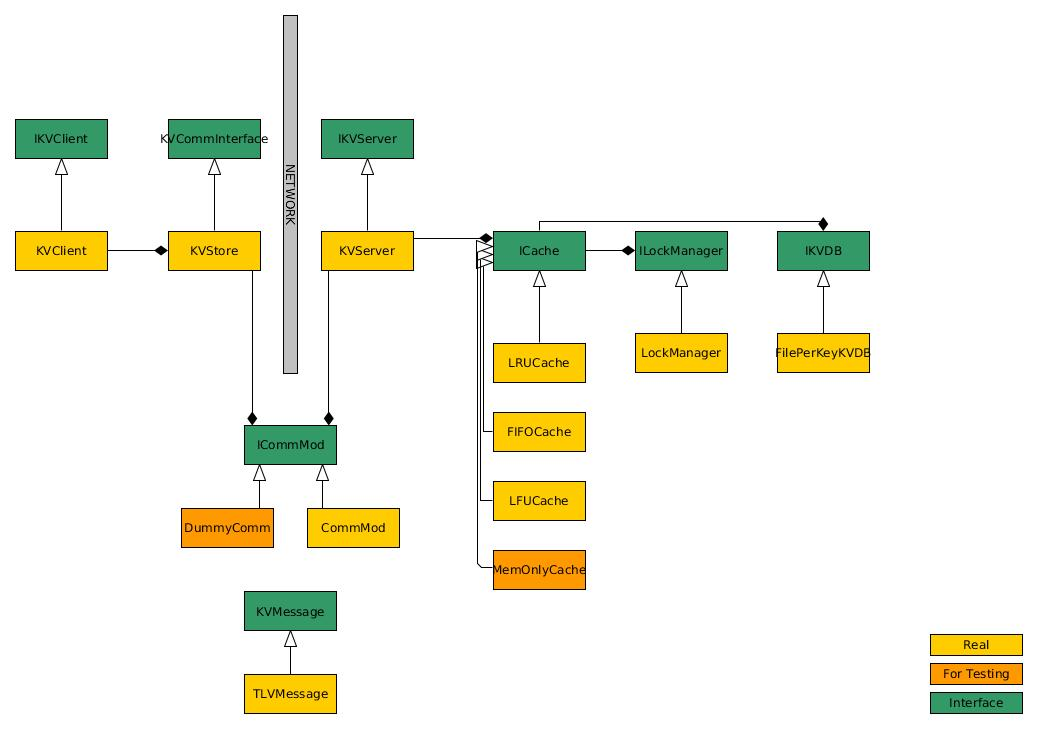
\includegraphics[scale=0.50]{architecture}
\caption{Architecture Diagram}
\label{arch}
\end{figure}
\end{document}

